\documentclass{emulateapj}
%\documentclass[12pt,preprint]{aastex}

\usepackage{graphicx}
\usepackage{float}
\usepackage{amsmath}
\usepackage{epsfig,floatflt}
\usepackage[toc,page]{appendix}
\usepackage{physics}
\usepackage{listings}
\usepackage{color}
\usepackage{hyperref}
\usepackage{cleveref}
\crefname{subsection}{subsection}{subsections}

% patch
\makeatletter
\usepackage{etoolbox}
\patchcmd\H@refstepcounter{\protected@edef}{\protected@xdef}{}{}
\makeatother

\lstset{language=Python}
\lstset{basicstyle=\small}
\lstset{backgroundcolor=\color{white}}
\lstset{frame=single}
\lstset{stringstyle=\ttfamily}
\lstset{keywordstyle=\color{red}\bfseries}
\lstset{commentstyle=\itshape\color{blue}}
\lstset{showspaces=false}
\lstset{showstringspaces=false}
\lstset{showtabs=false}
\lstset{breaklines}




\begin{document}

\title{On RGB color and monochromatic Charge-coupled device detectors}

\author{Jakob Borg}

\email{jakobbor@uio.no}

\altaffiltext{1}{Institute of Theoretical Astrophysics, University of
  Oslo, P.O.\ Box 1029 Blindern, N-0315 Oslo, Norway}
  
\begin{abstract}
  We explored the use of monochromatic CCD detectors for imaging in observational astronomy by recording and correcting a raw image of a single slit diffraction pattern. In addition we looked at some of the difficulties introduced when using a RGB color CCD without correcting for chromatic aberrations. For the correction process of the raw image multiple frames for bias, dark current and flat field where recorded and the contributed noise analyzed. From the flat frames, corrected for bias, the electron-to-ADU conversion factor of the camera was found to $79.228$. With this gain we found the readout noise from the detector in electrons to $34.357$. We found the normalized noise in composite flat field frames to decrease by the inverse square root of the number of pairs used, exactly as expected. The raw image was corrected by constructing a master flat field and a composite dark current frame. From the corrected image we calculated the width of the pixels in the CCD to be $6.308 \pm 0.2 \,\mu$m using the known properties of the diffraction pattern. The correction process did not remove the most substantial impurities in the raw image. This may be attributed to the poor way the flat field frames recorded, where we changed the optical path of the system too much.
\end{abstract}
\keywords{Color RGB CCD camera --- Monochromatic CCD camera --- Statistical analysis of noise and calibration data}

\section{Introduction}
\label{sec:introduction}
Historically many different mediums for capturing exposures in astronomical photography have been used, including film and different kinds of photographic plates. Whenever an exposure is captured some of the information from the incoming photons is lost in the process. Also noise and other limitations of the capturing method is introduced. This results in the exposure not representing the object we observe accurately. Understanding these limitations and sources of noise is crucial in astronomy, where we often observe very distant and faint objects, so that few of the initially emitted photons reach our telescopes and detectors.

Ever since Willard Boyle and George E. Smith invented the Charge-Coupled Device (CCD) in 1969 \citep{PattentCCD} they have become increasingly more popular in astronomy as our technology has improved. CCDs have an array of sensitive detectors that converts the energy of photons hitting them into electric charges quantified by electrons. These electrons can then be manipulated by potential wells which moves the charges to a register to be read. In addition to high accuracy, the CCD registers the exposures digitally. Each detector acts as a pixel in our image, where the amount of charge registered is proportional to the light intensity and may be converted to a pixel value using analog-to-digital units (ADU). This way it's easier to correct the raw image for noise and other limitations as well as perform statistical analysis and editing.

Some of the most important features in a detector is it's resolution, quantum efficiency, amount of thermal noise, spectral response, dynamical range and bit depth. With the steady improvement in technology over the years the CCDs have become extremely accurate for their cost and size compared to prior analog methods. We have made tinier and more versatile detectors, cheaper and cheaper. With smaller and more numerous pixels the maximum resolution has increased. The detectors also have a quantum efficiency approaching the maximum possible. Usually in the range of $90\%$ to $100\%$, so that as many of the photons as possible is registered. This efficiency is reached for a broad range of wavelengths as the spectral response of the detectors has improved. With a high linear dynamical range we can resolve details in both dim and bright parts of the signal at the same time. And with a high bit depth we can differentiate tiny deviations between neighboring pixels. All of these features makes the CCD cameras particularly useful in astronomy. They are in use in most of the modern space telescopes and observatories. 

In this paper our goal is first to explore some of the properties of a standard color CCD camera. Then we go through the process of taking a well exposed image using a monochromatic CCD camera, record calibration data and process the raw image to remove noise. The main focus will be oriented around the second part. As we will see, monochromatic cameras are most used in astronomy.

\section{Data and experimental setup}
\label{sec:data}
For the two cameras we used similar experimental setups, where we switch out a few key features. The main components are an externally powered light source projecting light through a filter piece and made parallel in a collimator tube. The parallel light then passes an aperture and is recorded in the camera. The cameras are controlled and output directly into a graphical user interface (GUI) on a computer.
\subsection{Exploring color CCD properties}
\label{subsec: Data/color CCD}
We used a white light lamp to produce light of different wavelengths in the visible spectrum. As filter piece we used a dampening filter to reduce the light intensity to not over expose the image or damage the camera. We used a singlet lens as aperture $7.3 \pm 0.2$ cm from the tube to focus the light onto a microscopic objective with a $M=20x$ magnifying effect. We recorded the exposure with a 8 bit color Edmund Optics USB camera. The camera properties are tuned to:
\begin{itemize}
\item Pixel clock: $24$ MHz
\item frame rate: $8.86$ fps
\item Exposure time: $4.794$ ms
\end{itemize}
Schematic of the setup in \cref{fig: Setup white}.
\subsection{Taking a well exposed monochromatic exposure}
\label{subsec: Data/mono CCD}
We used a red Helium-Neon laser with a wavelength of $\lambda = 635$ nm. To produce an image with interesting features to analyze we used a single slit with an opening $a = 100$ $\mu$m. The slit reduces the light intensity, so we also switched out the filter by an extension piece without filtering. The extension piece was of the same length as the dampening filter to minimize the change in the light path through the collimator tube. We used a 8 bit monochromatic Edmund Optics USB camera with an extension tube of length $L = 7.5 \pm 0.2$ cm attached to the lens. The slit was then placed in the opening of the tube projecting a diffraction pattern for the camera to record. 
The camera properties are tuned to:
\begin{itemize}
\item Pixel clock: $19$ MHz
\item frame rate: $3.92$ fps
\item Exposure time: $95.265$ ms
\end{itemize}
Schematic of the setup in \cref{fig: Setup red}.

\begin{figure}
	\centering
	\includegraphics[width=\linewidth]{./keynotes/exp_setup_white.pdf}
	\caption[Experimental setup white light]{Schematic of experimental setup for exploring camera properties of a RGB color CCD camera. The light intensity is reduced in the dampening filter so that the camera is able to differentiate the signal. The light is then made parallel in a collimator tube, and focused by the singlet lens producing an airy disc. The objective is placed in the focal plane of the lens to magnify the exposure for the camera. We can then observe the magnified airy disc on the computer screen.}
	\label{fig: Setup white}
\end{figure}

\begin{figure}
	\centering
	\includegraphics[width=\linewidth]{./keynotes/exp_setup_red.pdf}
	\caption[Experimental setup red light]{Schematic of experimental setup for taking well exposed image with a monochromatic CCD camera. The light is made parallel in a collimator tube, projected through a single slit to produce a diffraction pattern. The light is undisturbed through the extension tube of the camera and recorded. We can then observe the diffraction pattern on the computer screen.}
	\label{fig: Setup red}
\end{figure}


\section{Method}
\label{sec:method}
% Refer experimentation of camera properties to the appendix
\subsection{Color CCD experiment, singlet lens}
\label{subsec: Method/color CCD}
We calibrated the setup using a red laser to find the focal point of the thin singlet lens. Parallel light focused by a circular aperture produces an Airy disc \citep{lab1}, which we used to control the alignment of the lens in the optical axis. By requiring an even and circular Airy disc we minimized the effect of comatic aberrations, which occur if the plane of the lens is not normal to the optical axis.

After calibration we changed the light source to the mentioned white lamp and viewed the exposure on the GUI connected to the camera. Here we experimented with adjusting the cameras pixel clock, frame rate and exposure time to see how they effected the exposure.

The GUI allowed us to look at the registered pixel count in a slice of the image for each color red, green and blue (RGB) through a histogram. Due to chromatic aberrations, different wavelengths of light have different focal lengths, which is not accounted for by a singlet lens. Therefore we adjusted the position of the objective slightly back and forth to find the focal length of the different colors, defined by the point where we reached the highest registered intensity in RGB pixels. The maximum found pixel count in each color was measured using a ruler directly on the output screen and measuring the relative height of the peak in each color. Then the pixel count is calculated with uncertainties form the lengths. An example of how the histogram looked for the green maximum is included in appendix \ref{asec: Additional figures} \cref{fig: Pixel count green}.

\subsection{Monochromatic CCD experiment, single slit}
\label{subsec: Method/Record mono CCD}

\subsubsection{Well exposed image}
\label{subsubsec: Method/Well exposed image}
To make sure the image of the diffraction pattern was well exposed we tuned the camera properties to record the signal with as high intensity as possible to minimize the effect of noise. The optimal signal level is limited by the dynamical range and bit depth of the CCD, so that we don't over-expose the image. When the light intensity registered by a detector is exceeding the maximum pixel value in the bit depth, the information in the over-exposed pixel will be lost as it is truncated down to said maximum value. In addition, when very close to the maximum exposure level, the sensors might display a non-linear behavior in the quantum efficiency.

In our exposure of the diffraction pattern we are not concerned by the intensity in the center maximum, but rather the distance from the center to each minima and maxima of higher order. Therefor we calibrated the camera such that the pixel value registered for the first order maxima where about one half of the maximum. This way the center maximum of the image is over-exposed, but the features we are interested in are well exposed.

\subsubsection{Recording calibration data}
\label{subsubsec: Method/Calibration data}
We turned of the light source and removed the camera from the optical path of the setup. Then recorded multiple frames to be used for correcting the raw image for bias, dark current and flat field. For the correction frames we used the same pixel clock and frame rate as for the raw image, given in \cref{subsec: Data/mono CCD}, while adjusting the exposure time.

\paragraph{Flat field frames}
Flat field correction compensates for variations in quantum efficiency from pixel to pixel through the hole field of view, as well as imperfections in the optical path. We recorded $16$ basic flat field frames. Here we used a white sheet of paper held at an angle to reflect a uniform field of light from the ceiling into the camera. To do this we had to move the CCD camera out of the optical path of the system to face the white paper. We adjusted the exposure time to $0.762$ ms so that the average pixel value in the recording is about one-third of the maximum value.

\paragraph{Bias and dark current frames}
The bias and dark current frames are recorded in total darkness. The bias gives a measure of the lowest level in a signal. Ideally this level should correspond to a pixel value of $0$, but is set to a low positive value in order to account for the digitization noise. During the integration time of the exposure in the CCD a dark current is present from generation of extra thermal electrons in the system not due to detection of photons.

Both the bias and dark current exposures where recorded with the dust cover on the camera to reduce the signal as much as possible. We recorded 
\begin{itemize}
\item five dark frames with the same exposure as the flat fields, $0.762$ ms
\item five dark frames with the same exposure as the raw image, $95.265$ ms
\item one dark frame with maximum exposure time, $255.02$ ms
\item two bias frames with the minimum exposure time $0.169$ ms
\end{itemize}
 
\subsubsection{Statistical analysis of correction frames}
\label{subsubsec: Method/ Statistical on correction frames}
All of the statistical analysis are written in Python 2.7.14. The scripts are included in appendix \ref{asec: Python scripts}. With the images saved as bitmap files we read the files into two dimensional arrays, where each element in the array corresponds to one pixel with a given value $\in [0,\,255]$. Let $B_i$, $F_i$ and $D_i$ correspond to the arrays obtained from bias, flat field and dark current frame number $i$ respectively. Using the array representation of the images we can add and subtract them and perform numerical calculations by operating on the arrays.

\paragraph{Comparing bias and dark frame} 
First we compared one of the two bias frames $B_1$ with the dark current frame captured with maximum exposure $D_{max}$. We found the mean, minimum and maximum pixel values of the two frames. In addition we compared the coordinates of the maximum pixel in the arrays, and the distribution of the pixel values.

\paragraph{Mean value in composite frames}
The mean value of a frame is given by its expectation value. As the expectation value is linear it's trivial to find the mean of composite frames.
\begin{equation}
	\mu = E\qty[B_1 + B_2] = E\qty[B_1] + E\qty[B_2] = \overline{B}_1 + \overline{B}_2
	\label{eq: Composite mean}
\end{equation}

\paragraph{Noise in composite frames}
To model the noise in an image we used the standard deviation of the pixel values. By subtracting one correction frame from another, we find the change in pixel values due to random noise not constant in time. To avoid unwanted effects near the edges we extract the square central part of the image, with $300$ pixels on a side.

From the addition rules of variance for $n$ uncorrelated variables \citep{STKbok} we know the standard deviation should increase by a factor of $\sqrt{n}$. This relation is shown in \cref{eq: STD n variables} in appendix \ref{asubsec: Var uncorrelated shown}.

Using \cref{eq: Composite mean} we found the mean of the pixel values in the composite bias frame, $\overline{B}_1 + \overline{B}_2$. The non-static noise, $\sigma_{(B_1-B_2)}$, is found from the standard deviation. The same procedure on two of the flat frames gives $\overline{F}_1 + \overline{F}_2$ and $\sigma_{(F_1-F_2)}$.

\paragraph{Read out noise in electrons}
As the signal is converted to ADU, there is a conversion factor $g$ which relates the pixel counts to the actual number of measured electrons. The number of detected electrons are a positive discrete value, so we expect the signal to follow Poisson statistics \citep{STKbok} measured in electrons, such that $\sigma_{electrons} = \sqrt{F_{electrons}}$. As the signal is converted using $g$, our actual measurements are $g\sigma_{electrons} = \sqrt{gF_{electrons}}$. Solving for $g$ and correcting for bias and bias noise we found the value of the conversion factor by
\begin{equation}
	g = \frac{F_{electrons}}{\sigma_{electrons}^2} = \frac{\qty(\overline{F}_1 + \overline{F}_2) - \qty(\overline{B}_1 + \overline{B}_2)}{\sigma_{(F_1-F_2)}-\sigma_{(B_1-B_2)}}
	\label{eq: Conversion factor}
\end{equation}

Ideally, the only source of noise in a single bias frame is the read out noise (R.O.N.). Having found the noise for the combined frame we used the relation in \cref{eq: STD n variables} to find the noise in a single frame 
\begin{equation}
	\sigma_{B_1} = \frac{\sigma_{(B_1-B_2)}}{\sqrt{2}}
	\label{eq: Noise one bias}
\end{equation}

The R.O.N. in electrons was computed using the conversion factor and the noise from a single bias frame

\begin{equation}
	\text{R.O.N.} = g\sigma_{B_1}
	\label{eq: R.O.N.}
\end{equation}

\subsubsection{Normalized noise from composite frames}
\label{subsubsec: Method/Normalized noise}
By adding multiple pairs of correction frames we even out the random noise from each frame, but in the process amplify the static noise that overlap in multiple (or all) frames. To account for this we normalized the noise by the number of pairs used. The normalization of multiple frames results in a reduction in the noise by a factor of $\frac{1}{\sqrt{n}}$, as shown in appending \ref{asubsub: Normalized noise}. We calculated the normalized noise for successively more pairs of flat field frames. Then the normalized noise together with the theoretical expectation where plotted against the number of pairs and compared. 

\subsubsection{Correcting raw image}
In the process of correcting the raw image we used a combination of the same statistical methods used on the calibration frames. First we found the average of all the flat field frames and the dark current frames with the same exposure.
\begin{align*}
	F_{avg} &= \frac{\sum_{i=1}^16 F_i}{16} 
	\\
	D_{avg,F} &= \frac{\sum_{i=1}^5 D_{i,F}}{5}.
\end{align*}
We constructed a normalized master flat frame by correcting the average of the flat frames for dark current, and divide by the mean value of the master flat.
\begin{align*}
	F_{master} &= F_{avg} - D_{avg,F}
	\\
	F_{normed,\, master} &=  \frac{F_{master}}{\overline{F}_{master}}
\end{align*}
To correct the raw image for dark current we found the average dark frame taken with the same exposure as the raw image. Correction for flat field was done using the normalized master flat.
\begin{align}
	D_{avg,I} &= \frac{\sum_{i=1}^5 D_{i,I}}{5}	\notag
	\\
	I_{corrected} &= \frac{I_{raw}-D_{avg,I}}{F_{normed,\, master}} \label{eq: Corrected image}
\end{align}
where $I$ denotes the proper image captured of the diffraction pattern.

\subsubsection{Calculating the pixel width}
We used the corrected image to calculate the size of the pixels in the CCD camera. The diffraction pattern is characterized using the equation for a single slit \citep{lab1}
\begin{equation}
	m\lambda = a\sin(\theta)
	\label{eq: Single slit diffraction}
\end{equation}
where $\lambda$ is the wavelength, $a$ is the slit width and $m$ is the order of the minimum at angle $\theta$ from the center maximum. A sketch of the geometry is displayed in \cref{fig: Diffraction measurements}. The number of pixels $n_p$ with width $w_p$ to minimum $m=4$ was found numerically by the intensity in the corrected image. To do this we found a row along the image array crossing the trenches in the pattern with high mean value. To minimize the uncertainty in $n_p$ we found the number of pixels between the fourth order minima on both sides of the center and divided by $2$. Then the angle $\theta$ was found by $\tan(\theta) = \frac{n_pw_p}{L}$. We know the diffraction pattern is in the Fraunhofer regime \citep{Fraunhofer}, so we used the small angle approximation
\begin{equation}
	\tan(\theta) \approx \sin(\theta) \approx \theta \approx \frac{n_pw_p}{L}.
	\label{eq: Small angle}
\end{equation}
The width of the pixels was then calculated as
\begin{align}
	w_p &= \frac{Lm\lambda}{an_p} \label{eq: pixel width}
	\\
	\qq*{with uncertainty} \frac{\delta w_p}{w_p} &= \sqrt{\qty(\frac{\delta L}{L})^2+\qty(\frac{\delta n_p}{n_p})^2} \label{eq: pixel width unc}
\end{align}
where we neglect the uncertainties in $a$ and $\lambda$ as they are negligible compared to $L$ and $n_p$.

\begin{figure}
	\centering
	\includegraphics[width=\linewidth]{./keynotes/pixelwidthmeasurments.pdf}
	\caption[Measurements diffraction pattern]{Sketch of the geometry in the procedure for finding the pixel size. $L$ is the distance from the slit to the camera. $m$ is the order of the minimum an angle $\theta$ from the center maximum. The number of pixels, and hence the pixel size, can be found using \cref{eq: Single slit diffraction}.}
	\label{fig: Diffraction measurements}
\end{figure}

\section{Results}
\label{sec:results}
\subsection{Color CCD experiment}
\label{subsec: Result/ color exp}
\subsubsection{Experimenting with camera properties}
\paragraph{Pixel clock}
A low pixel clock value resulted in a bright high intensity signal, and vice versa.
\paragraph{Frame rate}
A low frame rate delayed how changes in the image where displayed, and also seemed to effect the intensity in the exposure.
\paragraph{Exposure time}
A high exposure time results in high intensity signal, and vice versa.

\subsubsection{Chromatic aberrations}
We found the red light to have focal point furthest from the camera, blue light closest and the green light in the middle. The maximum count for each color are found to
\begin{itemize}
	\item Red: $125 \pm 27$
	\item Green: $172 \pm 37$
	\item Blue: $27 \pm 6$
\end{itemize}
The captured images of the Airy disc is shown in \cref{fig: Airy disc}. The images taken at the focal point of each color is included in appendix \ref{asec: Additional figures}.

\begin{figure}
	\centering
	\includegraphics[width=0.7\linewidth]{./images/ex2/cali_white.pdf}
	\caption{The Airy disc formed from the singlet lens and captured using the color RGB CCD camera.}
	\label{fig: Airy disc}
\end{figure}
\subsection{Monochromatic experiment}
\label{subsec: Results/ mono exp}

\paragraph{Well exposed raw image}
Pixel count across the diffraction pattern in two slices of the raw image displayed in \cref{fig: pixel count rows}. Compared with the mean value of all the rows, row number 37 is a slice with maximum mean value and row number 116 has average mean value. The central square of the captured raw image is included in \cref{fig: Raw image central}. The full image is shown in appendix \ref{asec: Additional figures} \cref{fig: Raw hole}.

\paragraph{Analysis of calibrating frames}
Results from the statistical analysis of the calibration data presented in \cref{tab: Statistical values calibration}. Histogram of the distribution of pixels in \cref{fig: Histogram bias} and \cref{fig: Histogram dark max}. The images of the first bias frame and the dark current with max exposure are included in appendix \ref{asec: Additional figures}.

\paragraph{Read out noise}
Noise from a single bias frame in ADU is found to
\begin{equation}
	\sigma_{B_1} = 0.43365 \approx 0.434
\end{equation}

The conversion factor is found as
\begin{equation}
	g = 79.22801 \approx 79.228\, \qty[\text{electrons/ADU}]
\end{equation}

The R.O.N. in electrons from a single bias frame is found to
\begin{equation}
	\text{R.O.N.}  = 34.35707 \approx 34.357
\end{equation}

\paragraph{Normalized noise}
Normalized noise of successively more pairs of frames together with the expected values are included in \cref{fig: Normalized noise}.

\paragraph{Corrected image}
The central square final corrected image is shown in \cref{fig: Corrected image central}. The corrections done on the full image is included in appendix \ref{asec: Additional figures} \cref{fig: Corrected hole}. We also found the mean pixel value in the two frames to be
\begin{itemize}
	\item Raw image mean $=76.822$
	\item Corrected image mean $=68.492$ 
\end{itemize}

\paragraph{Pixel size}
\Cref{fig: Pixel size} shows the number of pixels between the two minima of 4th order, giving number of pixels from central maximum
\begin{equation}
	n_p = 302 \pm 5
	\label{eq: Amount of pixels}
\end{equation}
where we add a fair but substantial uncertainty to account for errors. Eq. (\ref{eq: pixel width}) gives a pixel width
\begin{equation}
	w_p = 6.308 \pm 0.2 \, \mu\text{m}
\end{equation}

% PIXEL ROWS
\begin{figure}
	\centering
	\includegraphics[width=\linewidth]{./pythonscripts/pixelrows.pdf}
	\caption[Pixel count two rows]{Pixel count in two slices across the diffraction pattern. The slices are picked based on the mean pixel count across the row. In the upper plot one of the rows with the maximum mean is displayed, and the lower plot shows one of the rows with average mean.}
	\label{fig: pixel count rows}
\end{figure}

% STATISTICAL CALIBRATION DATA
\begin{deluxetable}{lccccc}
\tablewidth{0pt}
\tablecaption{\label{tab: Statistical values calibration}}
\tablecomments{Statistical values found for calibration data. For frames noted with subscript $c$ only the central square region of the image is evaluated. The Index-column gives the coordinates $\qty(x,\,y)$ for the maximum value pixel. For hole frames: $x \in\qty[0,480]$ and $y \in\qty[0,752]$. For central regions: $x,\, y \in\qty[0,300]$.}
\tablecolumns{6}
\tablehead{Frame & $\mu$ & Min & Max & Index & $\sigma$ }
\startdata
$B_1$ & $8.535$ & $6$ & $19$ & $\qty[439,\, 427]$ &  \\
$D_{max}$ & $8.978$ & $6$ & $47$ & $\qty[214,\, 478]$ &  \\
$\qty(B_1 + B_2)_c$ & $17.127$ & $13$ & $25$ & $\qty[247,\, 244]$ & $0.613$ \\
$\qty(F_1 + F_2)_c$ & $178.648$ & $159$ & $198$ & $\qty[290,\, 175]$ & $1.554$
\enddata
\end{deluxetable}

% HIST BIAS1
\begin{figure}
	\centering
	\includegraphics[width=\linewidth]{./pythonscripts/hist_pixel_bias1.pdf}
	\caption[Distribution pixels bias 1]{The distribution of pixel values for bias frame 1 displayed in appendix \ref{asec: Additional figures} \cref{fig: Image bias frame}.}
	\label{fig: Histogram bias}
\end{figure}

% HIST DARK MAX
\begin{figure}
	\centering
	\includegraphics[width=\linewidth]{./pythonscripts/hist_pixel_darkmax.pdf}
	\caption[Distribution pixels dark current max exposure]{The distribution of pixel values for the dark current frame with maximum exposure displayed in appendix \ref{asec: Additional figures} \cref{fig: Image dark max frame}. Note the high max value along the x-axis. There are pixels counted here, but the scaling on the y-axis makes them not visible.}
		\label{fig: Histogram dark max}
\end{figure}

% NORMALIZED NOISE
\begin{figure}
	\centering
	\includegraphics[width=\linewidth]{./pythonscripts/noise_composite.pdf}
	\caption[Normalized noise]{The scaling of the normalized error in successively higher number of pairs of flat frames. The expected error is included.}
	\label{fig: Normalized noise}
\end{figure}

% RAW IMAGE
\begin{figure}
	\centering
	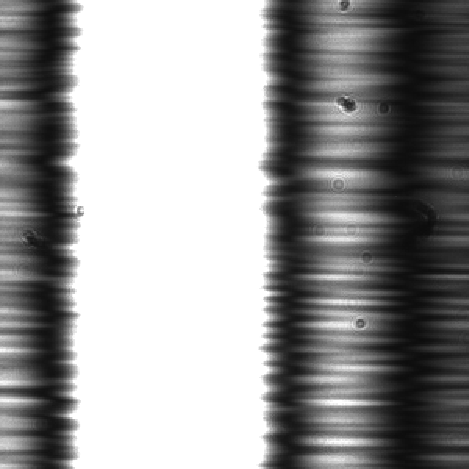
\includegraphics[scale=0.6]{./pythonscripts/raw_I.pdf}
	\caption[Raw image]{Central square part of raw image recorded of the diffraction pattern from \cref{subsec: Method/Record mono CCD}. Notice the imperfections in the optical path. There are dust obstructing the light which results in dark spots. The spots have light edges from the diffraction pattern formed by the shape of the particles. The corrected image is shown in \cref{fig: Corrected image central}.}
	\label{fig: Raw image central}
\end{figure}%

% CORRECTED IMAGE
\begin{figure}
	\centering	
	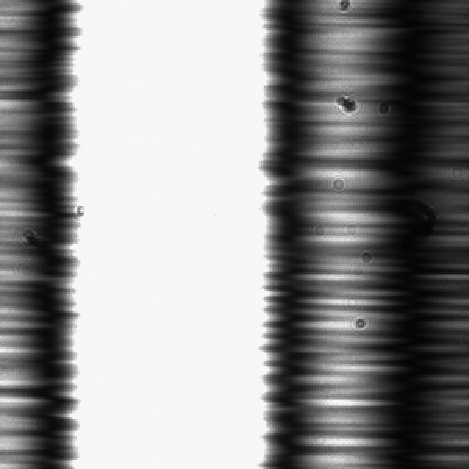
\includegraphics[scale=0.6]{./pythonscripts/corrected_I.pdf}
	\caption[Corrected image]{Central square part of the exposure of the diffraction pattern from \cref{subsec: Method/Record mono CCD} corrected with the dark current average and normalized master flat field. The raw image is shown in \cref{fig: Raw image central}.}
	\label{fig: Corrected image central}
\end{figure}

% PIXEL SIZE
\begin{figure}
	\centering
	\includegraphics[width=\linewidth]{./pythonscripts/pixellength.pdf}
	\caption[Counting pixels between minima]{The amount of pixels separating the two minima of 4th order. The slice of the image used has a high mean value.}
	\label{fig: Pixel size}
\end{figure}

\section{Conclusion and discussion}
\label{sec:conclusion}
\subsection{Color CCD}
The main point we want to emphasize by looking at the RGB camera is the draw backs of using a color CCD compared the a monochromatic CCD. As we have seen, when analyzing exposures in color one has to account for aberrations differently for each wavelength. In addition, each pixel in the exposure needs to detect and store information distributed between three colors, effectively acting as three pixels in one. This limits the sensitivity and versatility of the CCD compared to a monochromatic CCD and triples the amount of data one needs to store for each image.

Color might add esthetic values in an image, but we can determine color from the registered wavelength and edit in the colors later in the calibration process. Also, in astronomy we often want to observe light outside the visible spectrum. In these cases there are no conceptional meaning in separating the signal into red, green and blue pixels.

% MONOCHROMATIC
\subsection{Monochromatic CCD}
\label{subsec: Conclusion/ Monochromatic}

\subsubsection{Comparing calibration frames}
\label{subsubsec: Conclusion/ Comparing calibration frames}
% BIAS1 AND MAX DARK
\paragraph{Comparing bias with max exposure dark current}
The dark current and bias frames look similar, as seen in appendix \ref{asec: Additional figures}. Both frames are taken in total darkness, making them look black, but from the statistical analysis we note some differences.

The minimum pixel values are identical, as this is determined by the lowest signal level, but the maxima differ by a value of $28$. This is expected as the dark current frame is taken with maximum exposure time so the sensitive detectors records a higher pixel count due to more noise being generated. This is also evident in the mean, where the dark current have slightly higher value than the bias.

The maxima are also located differently in the two frames. We know the noise generated by dark current is random over the array of pixels, so the difference in maxima location and value are to be expected.

These differences can also be deduced by the histograms of the pixel values, although the details are illusive. Both frames have the majority of pixels with value $8$, so the higher value pixels is not shown as well. 

% NOISE BIAS AND FLAT
\paragraph{Composite frames}
For the composite bias frame we see as expected the mean and min values approximately double the value of a single frame. This is not the case for the max value, indicating that the max values in the two bias frames are not in the same pixel. This is not ideal as the bias frames should be close to identical, but the non-static noise in the frames are quite low so the standard deviation is low as to be expected.

The values for the composite flat frames are as expected much higher, as these frames is not captured in darkness but in a uniform, or close to uniform, light. We see the noise in the composite frame is quite larger than in the bias frames, which is probably due to the primitive way we captured the flat frames. Holding a white sheet of paper in hand is not stable enough from frame to frame to produce the exact same uniform field in each frame.  The distance from the field to the camera may change, as well as the plane of the paper shifting. Still, the normalized noise in composite flat frames decrease exactly as expected by the factor $\frac{1}{\sqrt{n}}$.
\paragraph{Conversion factor and read out noise}
From our value for the conversion factor we see that of approximately $80$ electrons the CCD register 1 ADU. This is quite poor compared to the detectors used in the wide field cameras aboard the Hubble Space Telescope \citep{HSTdetectors}, which has a conversion factor in the range $\qty[1.52,\, 1.56]$. This comparison is not so fair as we are comparing a standard cheap CCD with high end equipment with a much deeper potential well. The size of the potential well is important as a too high conversion factor over floods the potential wells so that registered electrons leaks out into neighboring pixels. Our camera would not handle the conversion factor used in the wide field cameras of the Hubble Space telescope, as the potential wells are far to shallow.

The read out noise gives us a measurement of noise generated in the integration time of the exposure. The R.O.N. in electrons are calculated using the conversion factor and noise from a single bias frame, which ideally is only the read out noise in ADU. The standard deviation in a single frame is found from the relation of variance from multiple variables, which should behave accurately as we saw for the noise in composite flat frames.  This means that $68\%$ (within one $\sigma$) of the exposures taken with the same setup have registered electrons deviating from the true mean of electrons by $34.357$. With a conversion factor of $79.228$ [electrons/ADU] this R.O.N. is very good, contributing with approximately $0.5$ ADU. This value seems low, and would be interesting to control in further detail in the future.\bigskip \bigskip

\subsubsection{Corrected raw image}
The correction process does not change the image significantly, but we can see a slight reduction in the intensity due to the random thermal noise from dark current in the raw image. This is corrected using the dark current frames, but as we have seen in the statistical analysis of the calibration data, the dark current generated is quite small. The correction is evident in the difference of $8.33$ in the mean value of the pixel count from the two images. In most of astronomical observations the raw exposures are prone to a much higher dark current being generated than in our simple setup, such that the correction for these effects are more important.

The most noticeable impurities in our raw image are the diffraction patterns and shadows resulting from the dust particles in the optical path. These obstructions should be corrected using the flat field frames. This is not the case, and is probably due to the poor quality of our flat fields as discussed under \cref{subsubsec: Conclusion/ Comparing calibration frames}. In addition to the flat fields not being uniform and constant over time, we changed the optical path of the system to capture the flat fields. By doing this we removed all the dust particles in the other instruments used along the path of the laser, so that the flat fields did not obtain the required information to correct for these impurities.

For future improvements we should take flat field correction frames in as close to the same optical path used for the proper image as possible. We should also use a much more stable source for the uniform field. In addition we could take more than 16 frames, as we have seen the noise in the flat fields decrease dramatically as we increase the number of pairs used.
\medskip

To conclude, the CCD is of huge importance in observational astronomy due to it's efficiency and applicability to multiple type of exposures. In addition to cameras, CCDs are in frequent use in many other instruments including spectrometers and interferometers. They provide good methods for recording correction data, without having to change the instrumental setup too much. In astronomy, and most other fields in physics, we tend not to use color CCDs as we get all relevant information from the wavelength of the light detected without the additional difficulties introduced by accounting for colors. With increasing technology the CCDs approaches the theoretical maximum in most of the key features we want in a detector, as well as being versatile, small, cheap and easy to operate.

\begin{acknowledgements}
  Thanks to my colleagues and co-workers in the execution of the experiments: Nils-Ole Stutzer, Jon Dahl and Barathy Pirabahar.\\
Thanks to our guide and supervisor in the lab: Ranghild Aurlien.
\end{acknowledgements}
\pagebreak
\bibliographystyle{plainnat}
\bibliography{ref}
\clearpage
\begin{appendices}
\section{Calculations}
\label{asec: Calculations}

\subsection{Variance and standard deviation of uncorrelated variables}
\label{asubsec: Var uncorrelated shown}
For $n$ variables with the same variance $V[X_i] = \sigma^2$, the variance of the sum of the variables \citep{STKbok} is given by
\begin{equation}
	V[a_1X_1 \pm a_2X_2 \pm \ldots \pm a_nX_n]  = a_1^2V[X_1] + a_2^2V[X_2] + \ldots + a_n^2V[X_n]
	\label{eq: Var n variables}
\end{equation}
if the weights $a_i = \pm 1$ for all $i$ this simplifies to
\begin{equation}
	\sigma_{(a_1X_1 \pm \ldots \pm a_nX_n)}^2 = \sum_{i=1}^n V[X_i]  = n \sigma^2
	\label{eq: Simplified Var n variables}
\end{equation}


We model the noise by the standard deviation of the difference of two frames, found by taking the square root of the variance of the difference. This means our weights are indeed $a_1=1$ and $a_2=-1$ so we can use the simplified expression
\begin{equation}
	\sigma_{(a_1X_1 \pm \ldots \pm a_nX_n)} = \sqrt{n\sigma^2} = \sqrt{n} \sigma
	\label{eq: STD n variables}
\end{equation}

\subsubsection{Normalized standard deviation of pairs of frames}
\label{asubsub: Normalized noise}
If we combine $n$ pairs of frames we know from \cref{eq: STD n variables} that the standard deviation should increase by a factor of $\sqrt{n}$. Normalizing by the number of pairs used
\begin{equation}
	\sigma_{composite, normed} =  \frac{\sqrt{n}}{n}\sigma = \frac{\sigma}{\sqrt{n}}
\end{equation}
results in a reduction in the noise a a factor $\frac{1}{\sqrt{n}}$.
\clearpage

\section{Additional figures}
\label{asec: Additional figures}
%BIAS AND DARK MAX IMAGE
\begin{figure}[h!]
	\begin{minipage}{.5\textwidth}
	\centering
	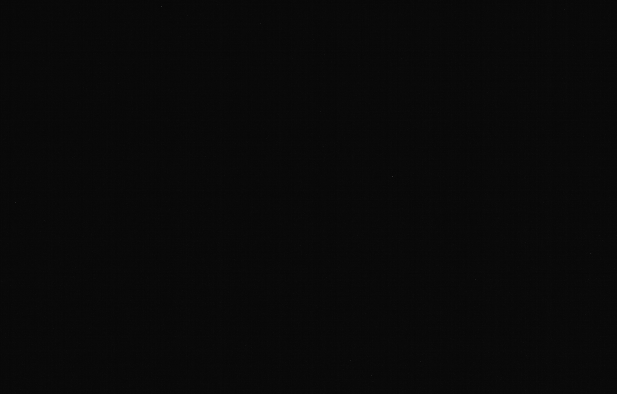
\includegraphics[width=0.8\linewidth]{./images/ex3_4_5/dark_max.pdf}
	\caption[Dark current correction frame with max exposure]{Image of dark current frame with max exposure.}
	\label{fig: Image dark max frame}
	\end{minipage}%
	\begin{minipage}{.5\textwidth}
	\centering
	
\includegraphics[width=0.8\linewidth]{./images/ex3_4_5/bias1.pdf}
	\caption[Bias correction frame 1]{Image of bias frame number 1.}
	\label{fig: Image bias frame}
	\end{minipage}
\end{figure}

%HOLE CORRECTED AND RAW
\begin{figure}[h!]
	\begin{minipage}{.5\textwidth}
	\centering
	\includegraphics[width=0.8\linewidth]{./pythonscripts/raw_i_hole.pdf}
	\caption[Hole raw image captured]{The hole raw image captured.}
	\label{fig: Raw hole}
	\end{minipage}%
	\begin{minipage}{.5\textwidth}
	\centering
	\includegraphics[width=0.8\linewidth]{./pythonscripts/corrected_i_hole.pdf}
	\caption[Hole corrected image]{Corrections on the hole raw image.}
	\label{fig: Corrected hole}
	\end{minipage}
\end{figure}

% CHROMATIC ABERRATIONS AND CALIBRATING RGB
\begin{figure}[h!]
	\begin{minipage}{.5\textwidth}
	\centering
	\includegraphics[width=0.8\linewidth]{pixelcount_green.pdf}
	\caption[Green max pixel count]{Example of finding max pixel count for RGB camera, here viewing the for green.}
	\label{fig: Pixel count green}
	\end{minipage}%
	\begin{minipage}{.5\textwidth}
	\centering
	\includegraphics[width=0.8\linewidth]{pixelcount_white.pdf}
	\caption[Pixel count white light]{Displaying the GUI and how the chromatic aberration separate each color, shown using max exposure time. In the lower right the histogram of pixel count for each color is included.}
	\label{fig: Pixel count white}
	\end{minipage}
\end{figure}

% RGB MAXING
\begin{figure}[h!]
	\begin{minipage}{.33\textwidth}
	\centering
	\includegraphics[width=0.7\linewidth]{./images/ex2/cali_red.pdf}
	\caption{Image captured when finding focal point for red light.}
	\end{minipage}%
	\begin{minipage}{.33\textwidth}
	\centering
	\includegraphics[width=0.55\linewidth]{./images/ex2/cali_green.pdf}
		\caption{Image captured when finding focal point for green light.}
	\end{minipage}%
	\begin{minipage}{.33\textwidth}
	\centering
	\includegraphics[width=0.6\linewidth]{./images/ex2/cali_blue.pdf}
		\caption{Image captured when finding focal point for blue light.}
	\end{minipage}
\end{figure}
\clearpage

\section{Python scripts}
\label{asec: Python scripts}
All codes are written in Python 2.7.14 and ran on macOS 10.14. All of the programs, the raw data, images and plots can also be found at 
\subsection{Calculating pixel count for RGB camera}
\lstinputlisting{./pythonscripts/RGBpixelcount.py}
\subsection{Analyzing first bias and dark frame}
\lstinputlisting{./pythonscripts/histogram_BIAS_max_dark.py}
\subsection{Mean and noise from combining two calibrating frames}
\lstinputlisting{./pythonscripts/mean_noise.py}
\subsection{Calculating and plotting normalized noise in flat fields}
\lstinputlisting{./pythonscripts/normalized_noise.py}
\subsection{Correcting final image and plotting pixel counts}
\lstinputlisting{./pythonscripts/clarification_raw.py}
\end{appendices}

\end{document}


\begin{deluxetable}{lccc}
%\tablewidth{0pt}
\tablecaption{\label{tab:results}}
\tablecomments{Summary of main results.}
\tablecolumns{4}
\tablehead{Column 1  & Column 2 & Column 3 & Column 4}
\startdata
Item 1 & Item 2 & Item 3 & Item 4
\enddata
\end{deluxetable}

